
\documentclass[a4paper,12pt]{article}

\usepackage{indentfirst}
\usepackage{cite}
\usepackage[utf8]{inputenc}
\usepackage[T1]{polski}
\usepackage{helvet}
\usepackage{graphicx}
\usepackage{svg}
\usepackage{color}
\usepackage{geometry}
\usepackage{float}
\usepackage{multirow}
\usepackage[hidelinks]{hyperref}
\usepackage{caption}
% dodaj bibliografię do spisu treści
\usepackage[nottoc]{tocbibind}
% unikaj pojedynczych linii na początku/ końcu stron
\usepackage[defaultlines=4,all]{nowidow}
\usepackage{subcaption}
\usepackage{amsmath}
\usepackage{amsfonts}

% set default figure placement to !htbp
\makeatletter
\def\fps@figure{!htbp}
\makeatother


\newcommand{\setSubtitle}[1]{
    \newcommand{\subtitle}{#1}
    }

\newcommand{\labdate}{28 listopada 2020}
\newcommand{\temat}{Mikroskop MET-3}

\begin{document}
    
% Please add the following required packages to your document preamble:
% \usepackage{multirow}
% \usepackage{graphicx}

\begin{table}[]
    \resizebox{\textwidth}{!}{%
    \begin{tabular}{|c|c|c|c|}
    \hline
    \multicolumn{2}{|c|}{\multirow{2}{*}{\hspace{0.5cm} 
\includegraphics[height=2.3cm]{img/logoAGH} \hspace{0.5cm} }}                                                                    & \multicolumn{2}{c|}{\textbf{\begin{tabular}[c]{@{}c@{}} Akademia Górniczo-Hutnicza w Krakowie\\ Wydział Inżynierii Materiałowe i Ceramiki  \vspace{0.5cm} \end{tabular}}}                                     \\ \cline{3-4} 
    \multicolumn{2}{|c|}{}                                                                                       & \multicolumn{2}{c|}{\begin{tabular}[c]{@{}c@{}}Aleksandra Barcz\\ Alicja Kotwica  \vspace{0.5cm} \end{tabular}}                                                                                              \\ \hline
    \multicolumn{4}{|c|}{\textbf{Metody Badań Materiałów}}                                                                                                                                                                                                                                                     \\ \hline
    \multicolumn{4}{|c|}{\textbf{\temat}}                                                                                                                                                                                                                                                                            \\ \hline
    \begin{tabular}[c]{@{}c@{}}Rok Akademicki:\\ 2020/2021\end{tabular}         & \multicolumn{2}{c|}{\begin{tabular}[c]{@{}c@{}}Rok studiów:\\ IV\end{tabular}}                                  & \begin{tabular}[c]{@{}c@{}}Kierunek:\\ Ceramika\end{tabular}                                                       \\ \hline
    \begin{tabular}[c]{@{}c@{}}Data wykonania ćwiczenia\\ \labdate \end{tabular} & \multicolumn{2}{c|}{\begin{tabular}[c]{@{}c@{}}Data oddania sprawozdania:\\ \today \end{tabular}} & \begin{tabular}[c]{@{}c@{}}Prowadzący:\\ Dr. inż. Beata Macherzyńska\end{tabular}                                  \\ \hline
    \end{tabular}%
    }
    \end{table}


\section{Cel ćwiczenia}

Celem ćwiczenia było zapoznanie się z~budową mikroskopu metalograficznego MET-3 do badań w~świetle odbitym, opanowanie sposobu jego ustawiania i~obsługi oraz zastosowanie mikroskopu do badań jakościowych i~ilościowych zgładów.

\section{Wprowadzenie}

Mikroskop metalograficzny typ MET-3 działa na zasadzie światła odbitego od próbki. Służy przede wszystkim do badań struktury powierzchni i~do sprawdzania surowców, np. w~przemyśle. Jego powiększenie wynosi nawet $400x$ przy zastosowaniu obiektywu $40x$ i~okularu $8x$ (oraz $1.5x$ z~powiększenia dwuocznej nasadki okularowej i~1,25 z~głowicy, jednooczna nasadka okularowa nie ma znaczenia, gdyż ma $1x$). Dzięki temu, że w~tym urządzeniu jest zastosowany transformator, można płynnie regulować natężenie strumienia świetlnego. 

Mikroskop ten jest bardzo zbliżony do tego o przechodzącej wiązce światła, główna różnica jest w~występowaniu głowicy, w~której znajduje się pryzmat lub zwierciadło płaskie. 
\newline
Uogólniając: 
\begin{itemize}
    \item źródło światła jest oddzielone kolektorem, aby nie doprowadzić do przegrzania i~pęknięć szkła,
    \item transformator też jest ustawiony na $4/5$ mocy, aby nie spalić żarówki,
    \item apertura jest regulowana, po przejściu przez kondensor promień idzie dalej przez obiektyw, odbija się od przedmiotu umieszczonego na stoliku, po czym znowu znajduje się w~obiektywie i~jest odbijany do tubusa i~okularu.
\end{itemize}

Ciemne miejsca powstają na skutek rozproszenia wiązki, która przez to nie może wrócić jako odbita i~widzialna. Im większe mamy przybliżenie tym mniejszy możemy obserwować wycinek przedmiotu. Ma to swoje zalety, ponieważ badanie powierzchni jest dokładniejsze, bo gdy przy mniejszym powiększeniu niektóre promienie nie wpadały lub była mniejsza zdolność rozdzielcza, to w~tym przypadku jest większa szansa na powrót i~tym samym znalezienie większej liczby niuansów. 

Ustawianie oświetlenia robi się według Koehlera, również ostrość jest ustawiania śrubą mikrometryczną i~makrometryczną. Obserwacji można dokonywać w~ciemnym i~jasnym polu widzenia. W~ciemnym jest większy kontrast, wiązka padająca na preparat jest pod większym kątem od kąta aperturowego obiektywu. Przez odchylenie promieni od swego kierunku obraz jest jasny z~ciemnym tłem. Ustawienie to jest zwłaszcza przydatne do żywych materiałów biologicznych. W~jasnym polu widzenia obraz jest płaski i~szczegółowy. Przy płaskim zwierciadle możliwe jest wykorzystanie pełnej apertury, ale przez to, że szkło jest półprzepuszczalne, to tracimy się na jasności, co innego, jeśli jest pryzmat, wtedy nie można wykorzystać pełnej apertury i~zdolność rozdzielcza spada. Często też wpływ na kontrast ma obserwacja w~świetle spolaryzowanym, z~kontrastem fazowym i~interferencyjnym oraz przy podwyższonych lub obniżonych temperaturach. 

Mniejsze przybliżenia, ale za to obraz 3D można uzyskać w~mikroskopie stereoskopowym, który też działa na światło odbite. Powiększenie to wynosi od $4x-100x$, zatem często nie jest on aż tyle używany do badań, co do prac przy wykonywaniu preparatów lub warsztatowych czynności. Dodatkowo jego obsługa jest prosta, bo powiększenie zmienia się pokrętłem, a~ostrość śrubą. Zgłady do obserwacji wymagają starannego przygotowania. Na początku jest zgrubne szlifowanie coraz to mniejszym rozmiarem ziaren, a~potem polerowanie zawiesiną dla wygładzenia nierówności. Ziarna muszą być też dobierane, bo nie raz jak mają ostre krawędzie, np. $SiC-Si$ to może dochodzić w~niektórych materiałach do wyrywania cząstek. Ze zgładu można nie tylko określić zgrubny ogląd, ale również wyznaczyć ilościowe udziały faz np. metodą punktową.

\section{Aparatura i~materiały}

Wykorzystana aparatura:
\begin{itemize}
    \item Mikroskop do światła odbitego MET-3
    \item Mikroskop stereoskopowy MST-131
\end{itemize}
\newpage
Materiały wykorzystane w~badaniach:
\begin{itemize}
    \item EGH
    \item Grafit
    \item Ferryt
    \item Płytka krzemowa
    \item $SiC$
    \item $SiC-Si$
    \item Beton
    \item Włókna szklane w~żywicy epoksydowej
\end{itemize}

\section{Wyniki i~ich dyskusja}

\subsection{Przygotowanie mikroskopu do badań.}

Jako przygotowanie mikroskopu do badań, w~pierwszym kroku ustawiliśmy oświetlenie wg. zasady Kohlera.
W tym celu postępowaliśmy według następujących kroków:
\begin{itemize}
    \item Przygotowaną próbkę umieściliśmy na stoliku.
    \item Pod badaną próbką ustawiliśmy obiektyw $8x$ oraz wsunęliśmy do nasadki tubusa okular.
    \item Włączyliśmy oświetlenie.
    \item Otworzyliśmy przesłonę pola za pomocą pierścienia.
    \item Patrząc przez okular i~obracając pokrętką ruchu zgrubnego, później ruchu drobnego ustawiliśmy ostrość obserwowanego obrazu badanej próbki.
    \item Zmniejszyliśmy otwór przesłony pola, w~taki sposób, aby jej obraz był nieco mniejszy od pola widzenia.
    \item Wyjęliśmy okular z~tubusa.
    \item Nieznacznie przesuwając oświetlacz względem podstawy, uzyskaliśmy ostry obraz włókna żarówki.
    \item Zmniejszyliśmy do około $2/3$ wielkości średnicy wyjściowej obiektywu obraz przysłony aperturowej.
    \item Ponownie wsunęliśmy okular do tubusa i~ponownie ustawiliśmy ostrość obrazu, tym razem tylko za pomocą pokrętki ruchu drobnego.
\end{itemize}

\subsection{Opis ćwiczenia.}

Następnym krokiem po przygotowaniu mikroskopu do badań było zidentyfikowanie 6 różnych próbek (zdjęcie identyfikacji w~załącznikach), stworzonych z~innych materiałów (grafit, $EGH$, $SiC$, $SiC-Si$, ferryt, płytka krzemowa) i~wykonanie schematycznego rysunku czterech z~nich pod powiększeniem $8x$ oraz czterech pod powiększeniem $40x$. Kolejnym naszym zadaniem było zbadanie udziału objętościowego faz w~ferrycie. Aby było to możliwe, wykorzystaliśmy specjalne obiektywy z~wykalibrowaną siatką. 
Zliczaliśmy liczbę przecięć linii poziomych i~pionowych w~każdej z~faz z~osobna, na powiększeniu $8x$, a~następnie bez poruszania próbką, na powiększeniu $40x$.

\subsection{Obliczenia.}

Dokonaliśmy obliczeń powiększenia mikroskopu, z~wykorzystaniem powiększeń $8x$ i~$40x$. W~tym celu wykorzystaliśmy wzór:

$$p=p_{gł}\cdot p_{ob}\cdot p_{ns}\cdot p_{ok}$$

gdzie:
\newline
$p_{gł}$ - powiększenie głowicy
\newline
$p_{ob}$ - powiększenie obiektywu
\newline
$p_{ns}$ - powiększenie nasadki okularu
\newline
$p_{ok}$ - powiększenie okularu
\newline

Dla powiększenia $8x$: 
$$p_{8x}=1.25\cdot 8\cdot 1\cdot 10=100$$

Dla powiększenia $40x$:
$$p_{40x}=1.25\cdot 40\cdot 1\cdot 10=500$$

Schematyczne rysunki, wraz z~załączonymi zdjęciami ich realnych odpowiedników, znajdują się w~załącznikach wyników (na końcu sprawozdania).
\newline

Kolejnym naszym zadaniem było policzenie udziału objętościowego porów w~ferrycie. Badanie to wykonywaliśmy dwukrotnie, przez dwie różne osoby, w~dwóch różnych miejscach próbki. Zliczone liczby porów w~ferrycie przedstawia poniższa tabela. Aby wyliczyć udział objętościowy, wykorzystaliśmy wzór:
$$U_{obj}=\cfrac{L_p}{L_l} \cdot 100\%$$
\newline

gdzie:
\newline
$L_p$ - Liczba porów na skrzyżowaniu linii
\newline
$L_l$ - Liczba skrzyżowanych linii

% Please add the following required packages to your document preamble:
% \usepackage{graphicx}
\begin{table}[H]
    \caption{Liczba porów zliczona przez osobę numer 1.}
    \resizebox{\textwidth}{!}{%
    \begin{tabular}{|c|c|c|c|}
    \hline
    \multicolumn{2}{|c|}{Powiększenie 8x}           & \multicolumn{2}{c|}{Powiększenie 40x}           \\ \hline
    Lp.                 & Ilość porów w danej linii & Lp.                 & Ilość porów w danej linii \\ \hline
    1                   & 4                         & 1                   & 5                         \\ \hline
    2                   & 4                         & 2                   & 3                         \\ \hline
    3                   & 5                         & 3                   & 4                         \\ \hline
    4                   & 6                         & 4                   & 3                         \\ \hline
    5                   & 5                         & 5                   & 2                         \\ \hline
    6                   & 8                         & 6                   & 2                         \\ \hline
    7                   & 5                         & 7                   & 1                         \\ \hline
    8                   & 5                         & 8                   & 3                         \\ \hline
    9                   & 4                         & 9                   & 4                         \\ \hline
    10                  & 3                         & 10                  & 2                         \\ \hline
    11                  & 6                         & 11                  & 2                         \\ \hline
    Suma                & 37                        & Suma                & 31                        \\ \hline
    Udział objętościowy & 47\%                      & Udział objętościowy & 26\%                      \\ \hline
    \end{tabular}%
    }
    \end{table}
% Please add the following required packages to your document preamble:
% \usepackage{graphicx}
\begin{table}[H]
    \caption{Liczba porów zliczona przez osobę numer 2.}
    \resizebox{\textwidth}{!}{%
    \begin{tabular}{|c|c|c|c|}
    \hline
    \multicolumn{2}{|c|}{Powiększenie 8x}           & \multicolumn{2}{c|}{Powiększenie 40x}           \\ \hline
    Lp.                 & Ilość porów w danej linii & Lp.                 & Ilość porów w danej linii \\ \hline
    1                   & 4                         & 1                   & 4                         \\ \hline
    2                   & 4                         & 2                   & 1                         \\ \hline
    3                   & 6                         & 3                   & 3                         \\ \hline
    4                   & 4                         & 4                   & 2                         \\ \hline
    5                   & 4                         & 5                   & 2                         \\ \hline
    6                   & 3                         & 6                   & 1                         \\ \hline
    7                   & 5                         & 7                   & 1                         \\ \hline
    8                   & 5                         & 8                   & 2                         \\ \hline
    9                   & 5                         & 9                   & 2                         \\ \hline
    10                  & 5                         & 10                  & 1                         \\ \hline
    11                  & 4                         & 11                  & 2                         \\ \hline
    Suma                & 49                        & Suma                & 21                        \\ \hline
    Udział objętościowy & 40\%                      & Udział objętościowy & 17\%                      \\ \hline
    \end{tabular}%
    }
    \end{table}

\subsection{Opis naszkicowanych próbek.}

Grafit, dobrze przewodzi prąd elektryczny i~ciepło, jest odporny na wysoką temperaturę, kruchy. Ma znaczenie naukowe – służy do określania genezy skał metamorficznych, do wyrobu suchych smarów, do wyrobu cegieł ogniotrwałych, grafit do ołówków, czarne farby chroniące ołów przed korozją, naczynia ognioodporne, elektrody, jako zbrojenie materiałów kompozytowych, trzonki kijów golfowych typu driver, tygle ogniotrwałe, część ślizgowa pantografów, środki polerskie, jest dobrym moderatorem neutronów stosowanym w~reaktorach jądrowych.

Płytka krzemowa jest to cienka płytka monokrystalicznego krzemu. Ma zastosowanie  do wytwarzania czipów krzemowych (mikroprocesorów, mikrokontrolerów i~innych układów scalonych), ogniw słonecznych oraz mikroukładów elektromechanicznych.

Węglik krzemu bywa stosowany do pokrywania powierzchni ciernych pracujących w~wysokich temperaturach, na przykład powierzchni bocznych cylindrów silników, a~także jako osłony termiczne w~pojazdach kosmicznych. Jednym z~najnowszych zastosowań węgliku krzemu jest produkcja tranzystorów mikrofalowych.

Ferryty wytwarza się zazwyczaj przez spiekanie sproszkowanych tlenków metali we właściwych proporcjach. Stosuje się je do wyrobu rdzeni ferrytowych (anten ferrytowych), magnesów trwałych, pamięci ferrytowych i~innych elementów magnetycznych. Ferryty są to elementy wykonane ze związków tlenków żelaza z~dodatkiem pierwiastków takich jak: kobalt, nikiel, cynk oraz ziem rzadkich.
\newline
Cechą charakterystyczną ferrytów jest bardzo duża rezystancja, wynikająca z~budowy: sproszkowane metale połączone poprzez spiekanie z~nieprzewodzącym wypełniaczem, będącym jednocześnie lepiszczem. Ze struktury wewnętrznej ferrytu wynikają również małe prądy wirowe i~małe straty elektryczne. Efektem małych strat na przemagnesowanie jest duża impedancja ferrytu. Pasmo częstotliwości stosowania rdzeni zawierają się w~przedziale od kilku kHz do ponad 1 GHz. Zaletą stosowania ferrytów jest obniżenie stromości narastania przebiegów i~redukcja poziomu zakłóceń (przewodzonych, jak i~promieniowanych).

\section{Podsumowanie i~wnioski}

Powiększenie mikroskopu MET-3 pozwala na obejrzenie poszczególnych faz w~celu rozpoznania materiału, ale jeśli byłoby więcej próbek o bardzo drobnym uziarnieniu, takim jak w~$SiC$ mógłby nastąpić problem. Należy też dodać, że znaleźliśmy charakterystyczny dla tego materiału kwadratowy przekrój kryształu. Klasyczne cechy dla materiału takie jak ścieżki w~płytce krzemowej oraz włókna i~pory były dobrze widoczne. Przy zwiększeniu powiększenia z~$8x$ do $40x$ drobne ziarna $SiC$ stały się bardziej zauważalne, ale znalezienie dużych kryształów było trudne, ścieżki w~płytce krzemowej mogły być pomylone z~włóknami. Pomimo strat atrybutów zyskano więcej informacji o porach. Udział porów dla większego przybliżenia okazał się mniejszy, wynika to z~tego, że mogło dostać się więcej światła odbitego z~przedmiotu do obiektywu. Trzeba też przyznać, że metoda ta jest mało dokładna, bo wyniki pochodzące od dwóch osób znacznie się różniły (w $40x$ o $9\%$, a~w $8x$ o $7\%$). W~praktyce dla dokładnych danych liczy się pola powierzchni komputerowo lub rzadziej ręcznie. Nie mniej jednak metoda zliczania przecięć pozwala na całkiem dokładny i~w miarę szybki wynik, przy braku potrzeby większych szkoleń dla pracowników oraz przy relatywnie niskiej cenie sprzętu. Na koniec oglądaliśmy obraz z~mikroskopu stereoskopowego i~widok z~niego był przestrzenny i~pełny, niestety nie można było na nim uzyskać zbyt dużych powiększeń (może mieć nawet powiększenia tożsame z~lupą).

\section{Załączniki wyników}

\begin{figure}[H]
    \begin{subfigure}{.5\textwidth}
        \centering
        % include first image
        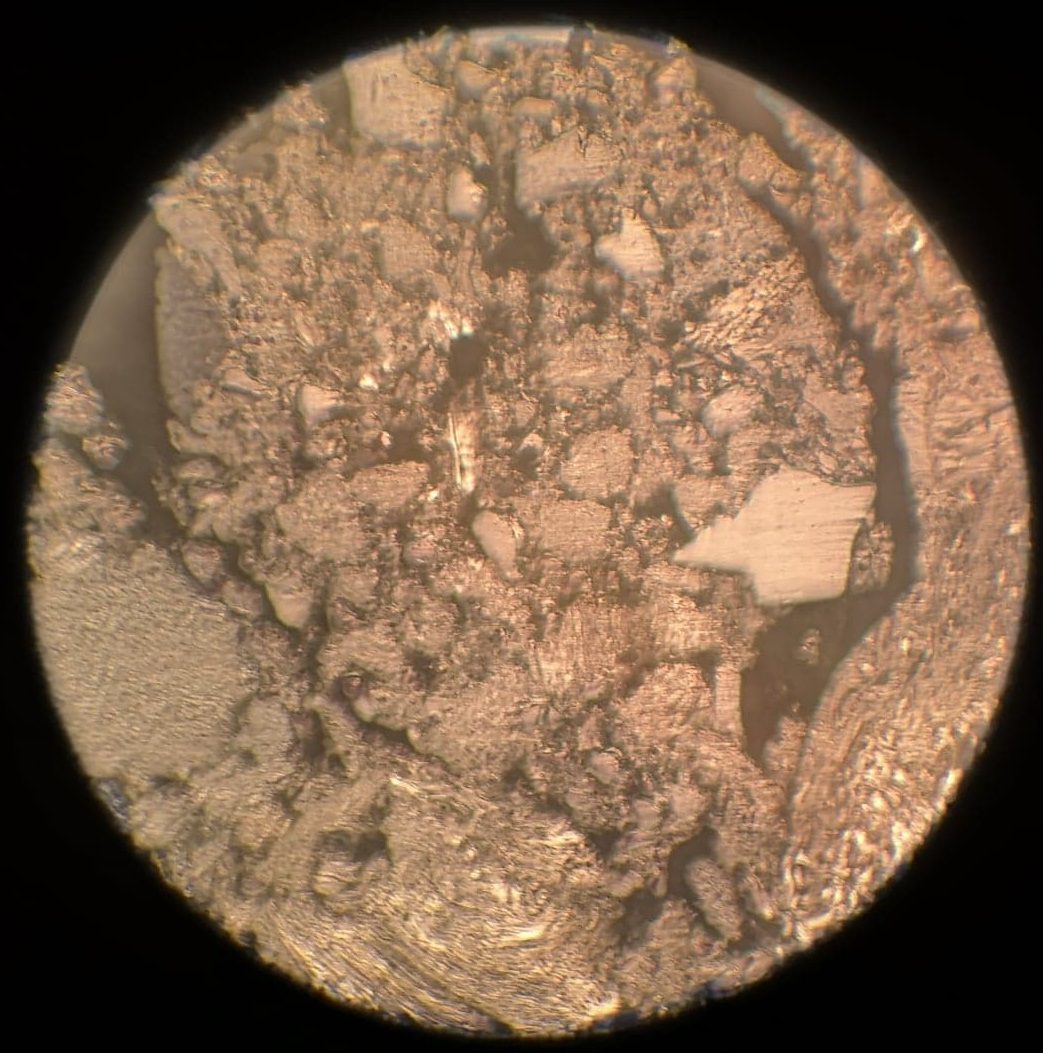
\includegraphics[width=.8\linewidth]{img/EGH8.jpg}  
        \caption{Powiększenie $8x$}
    \end{subfigure}
    \begin{subfigure}{.5\textwidth}
        \centering
        % include second image
        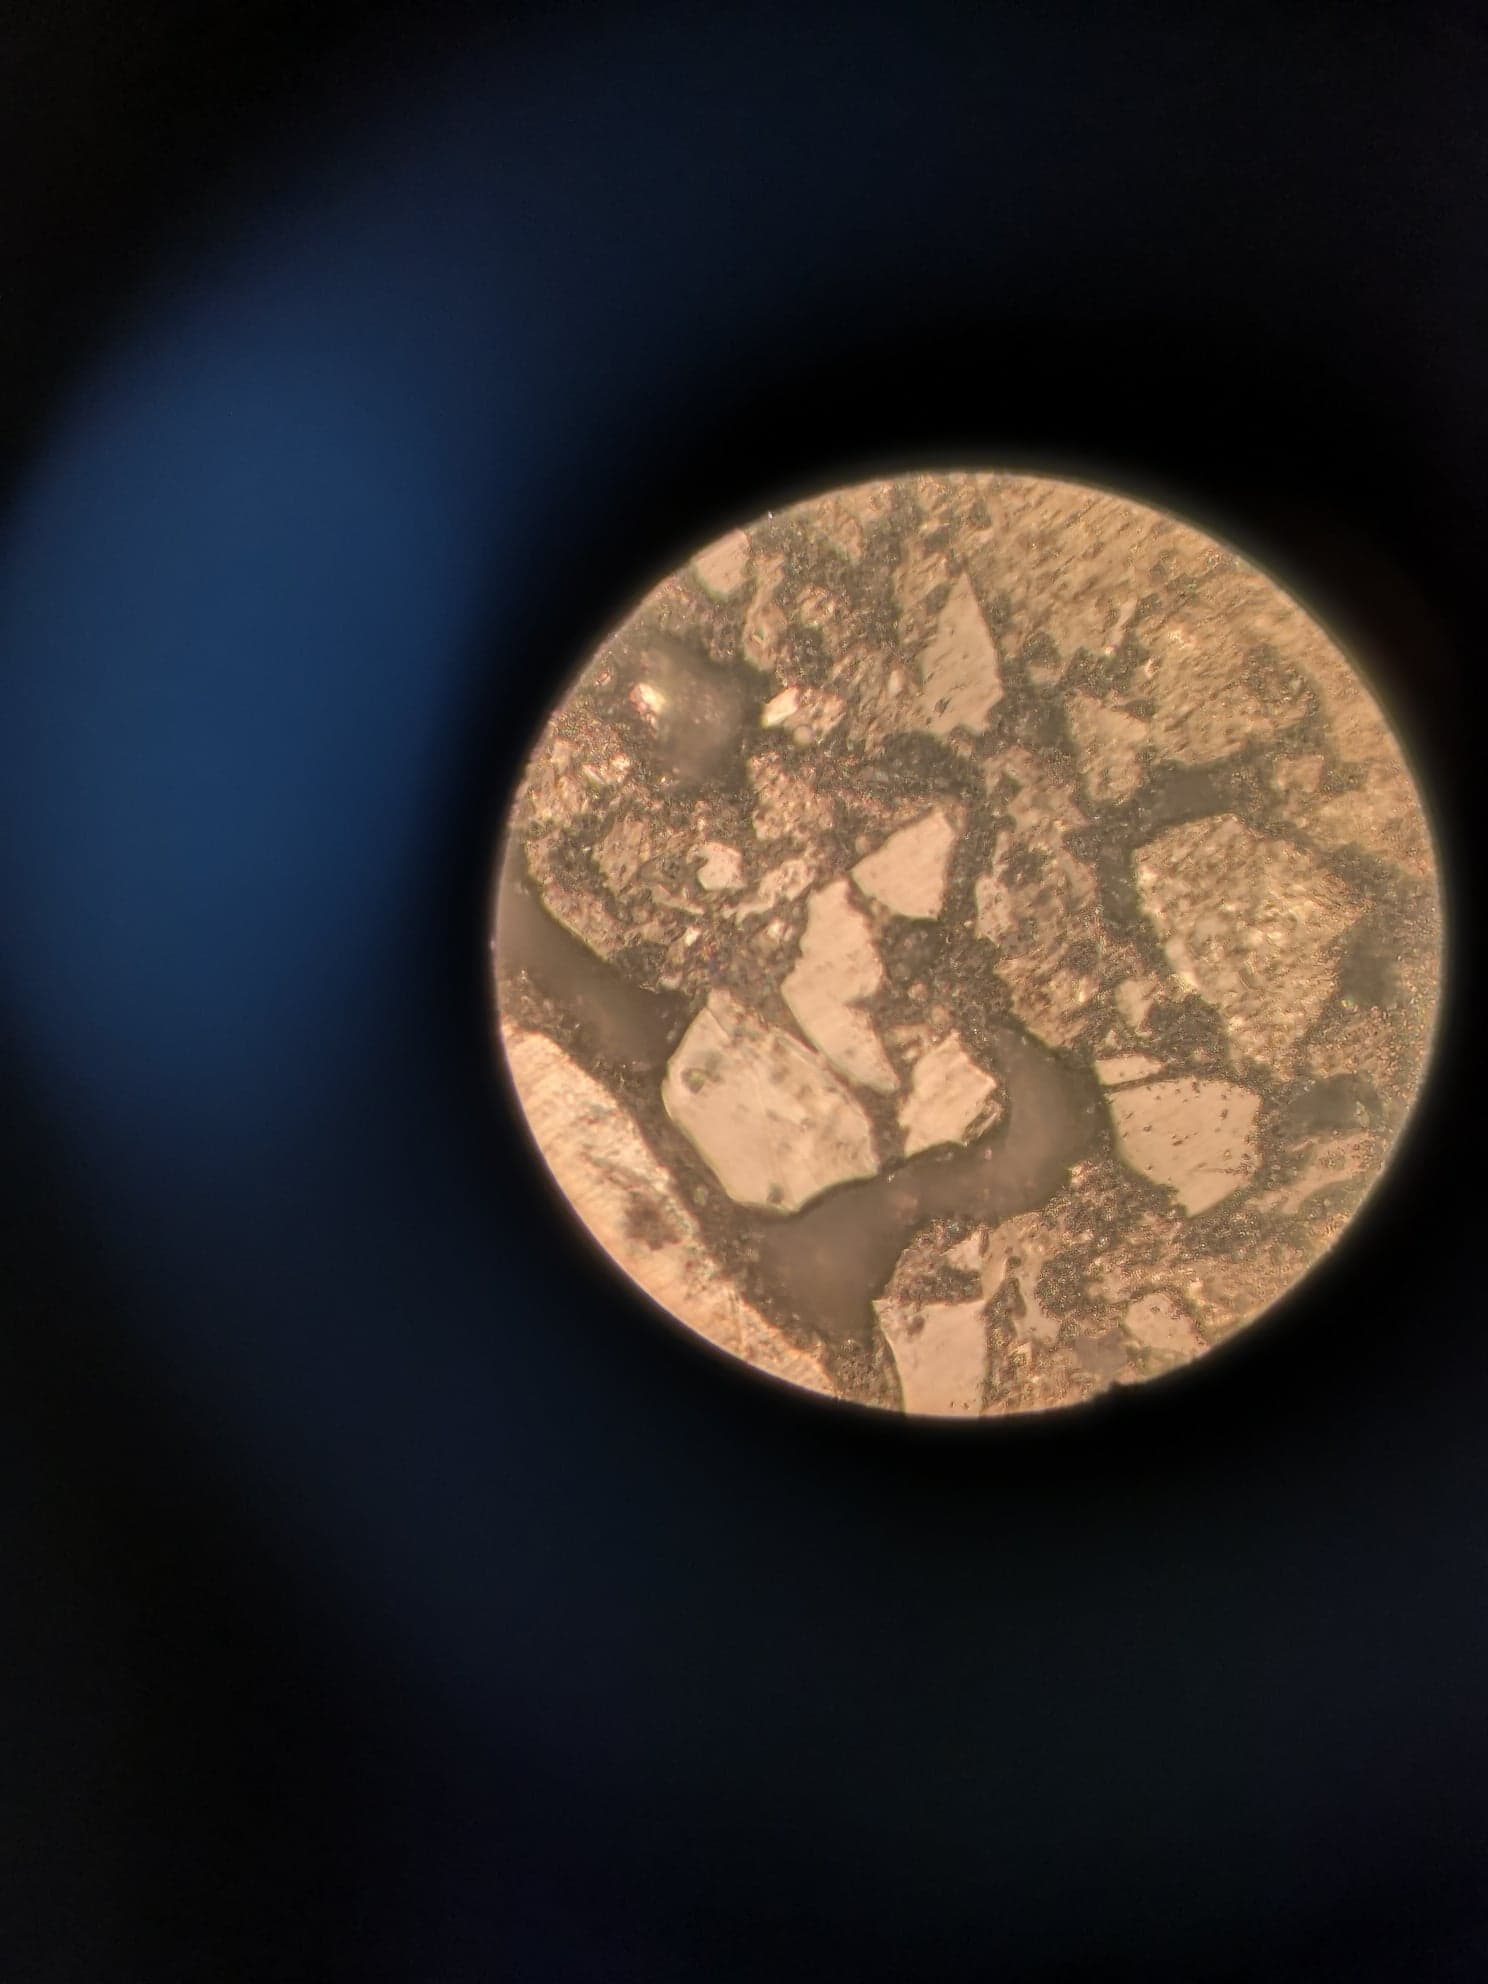
\includegraphics[width=.8\linewidth]{img/EGH40.jpg}  
        \caption{Powiększenie $40x$}
    \end{subfigure}
    \caption{EGH}
\end{figure}

\begin{figure}[H]
    \begin{subfigure}{.5\textwidth}
      \centering
      % include first image
      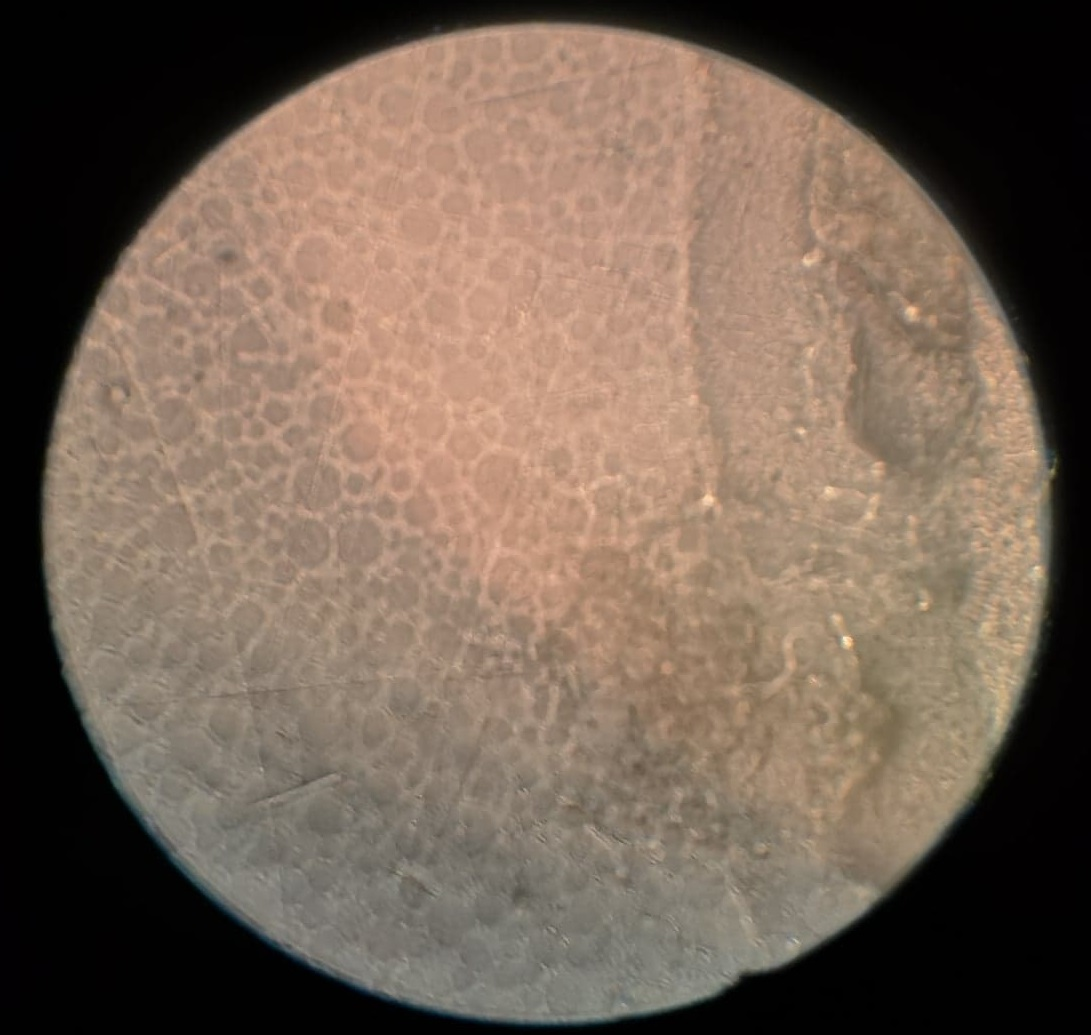
\includegraphics[width=.8\linewidth]{img/grafit8.jpg}  
      \caption{Powiększenie $8x$}
    \end{subfigure}
    \begin{subfigure}{.5\textwidth}
      \centering
      % include second image
      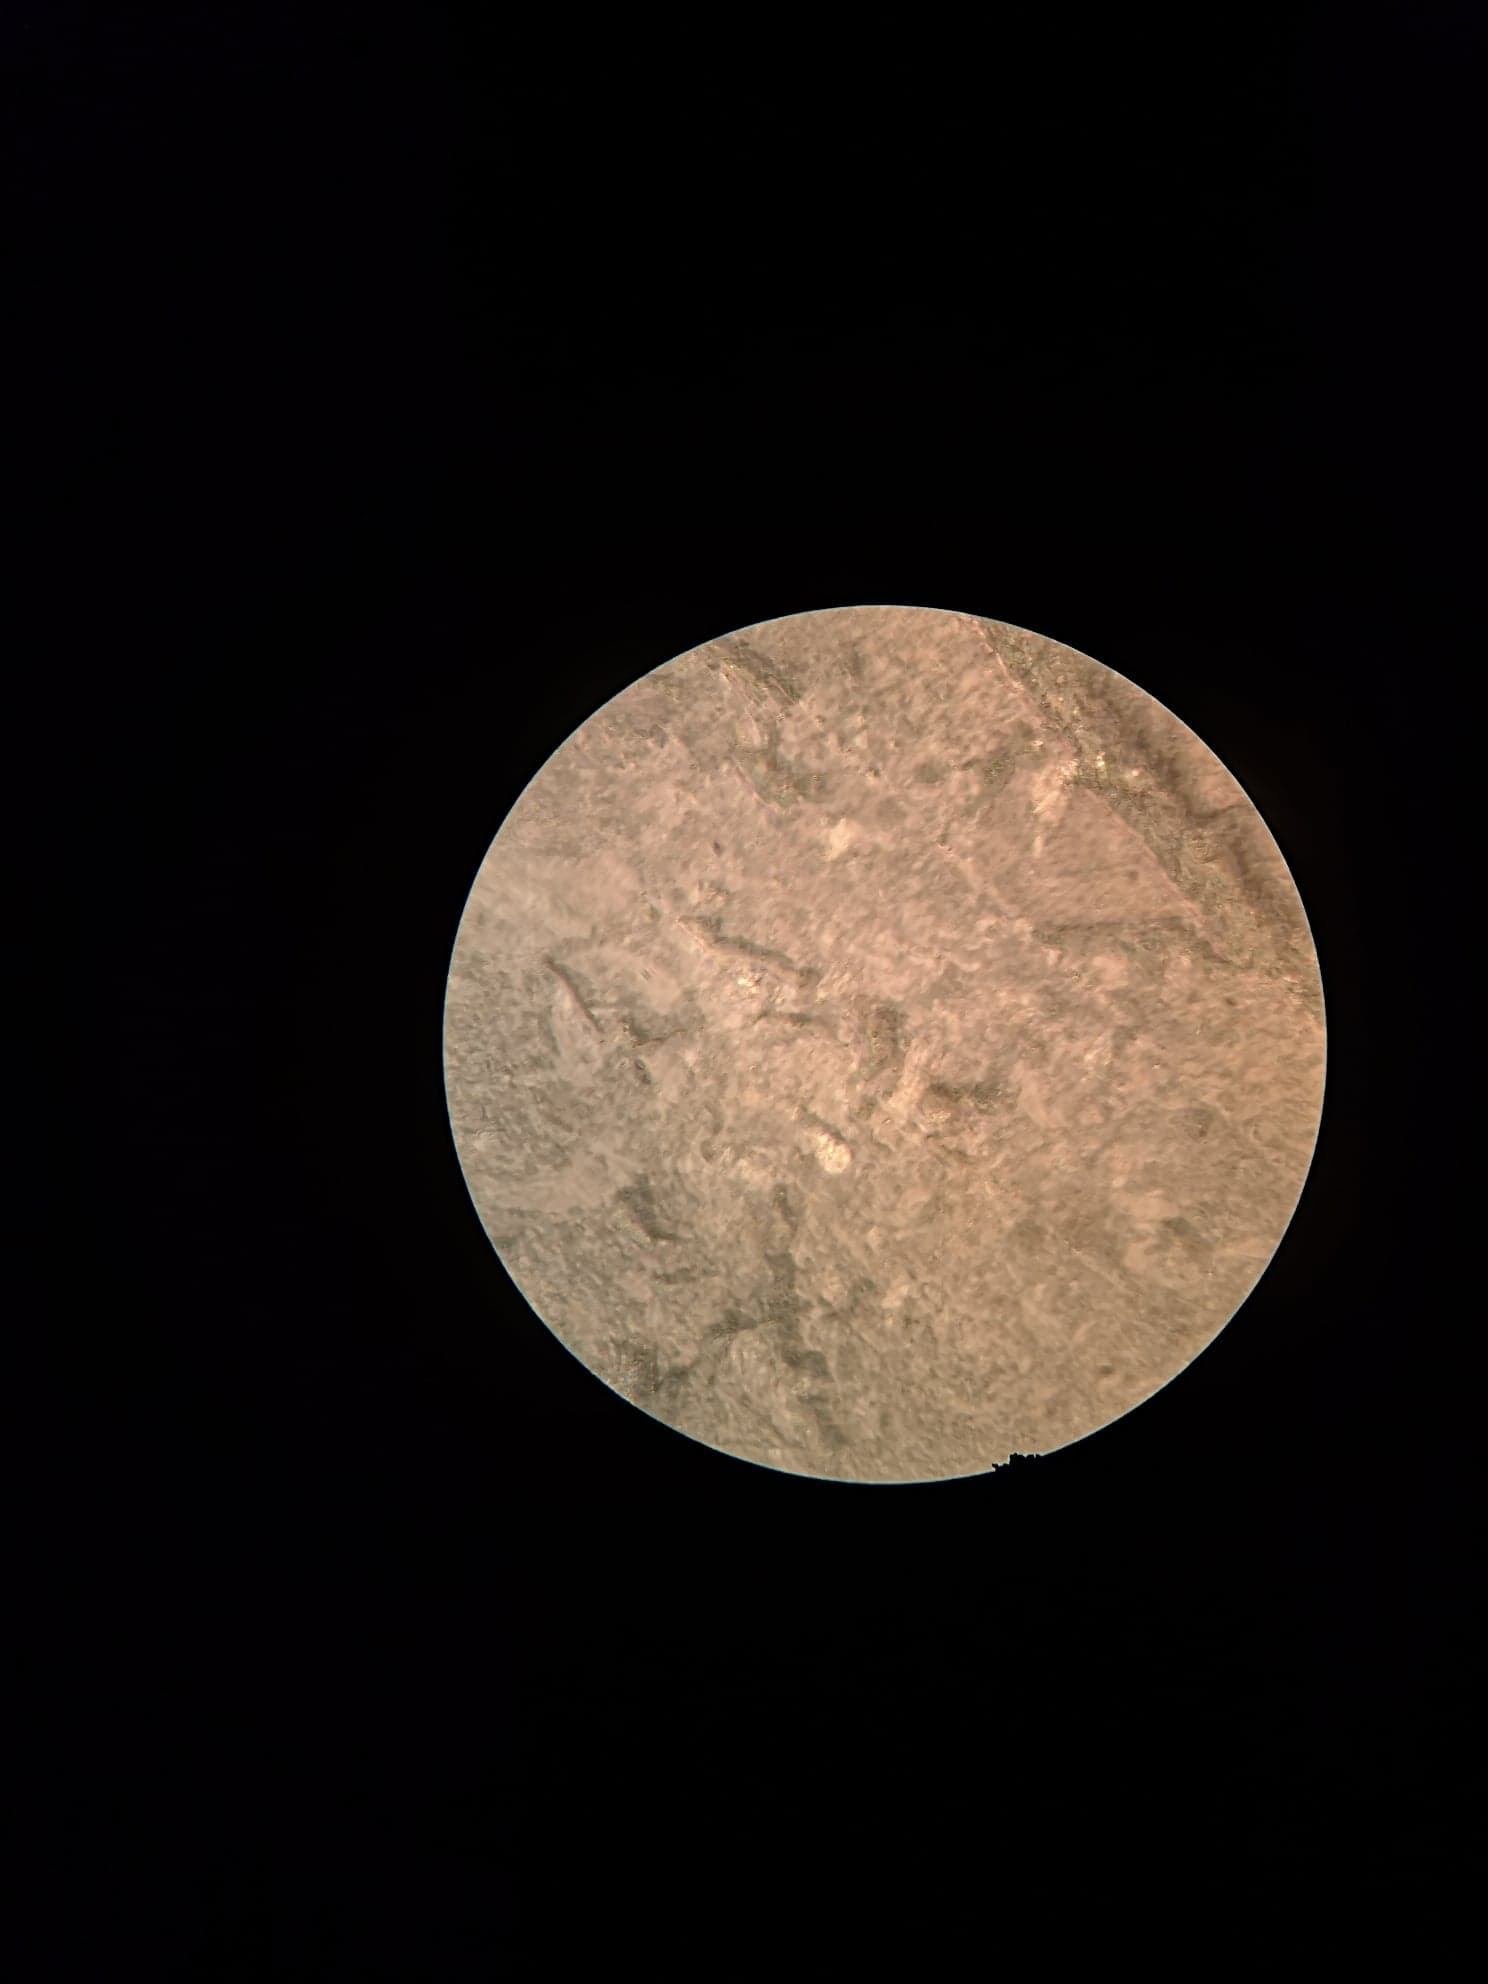
\includegraphics[width=.8\linewidth]{img/grafit40.jpg}  
      \caption{Powiększenie $40x$}
    \end{subfigure}
    \caption{Grafit}
\end{figure}

\begin{figure}[H]
    \begin{subfigure}{.5\textwidth}
        \centering
        % include first image
        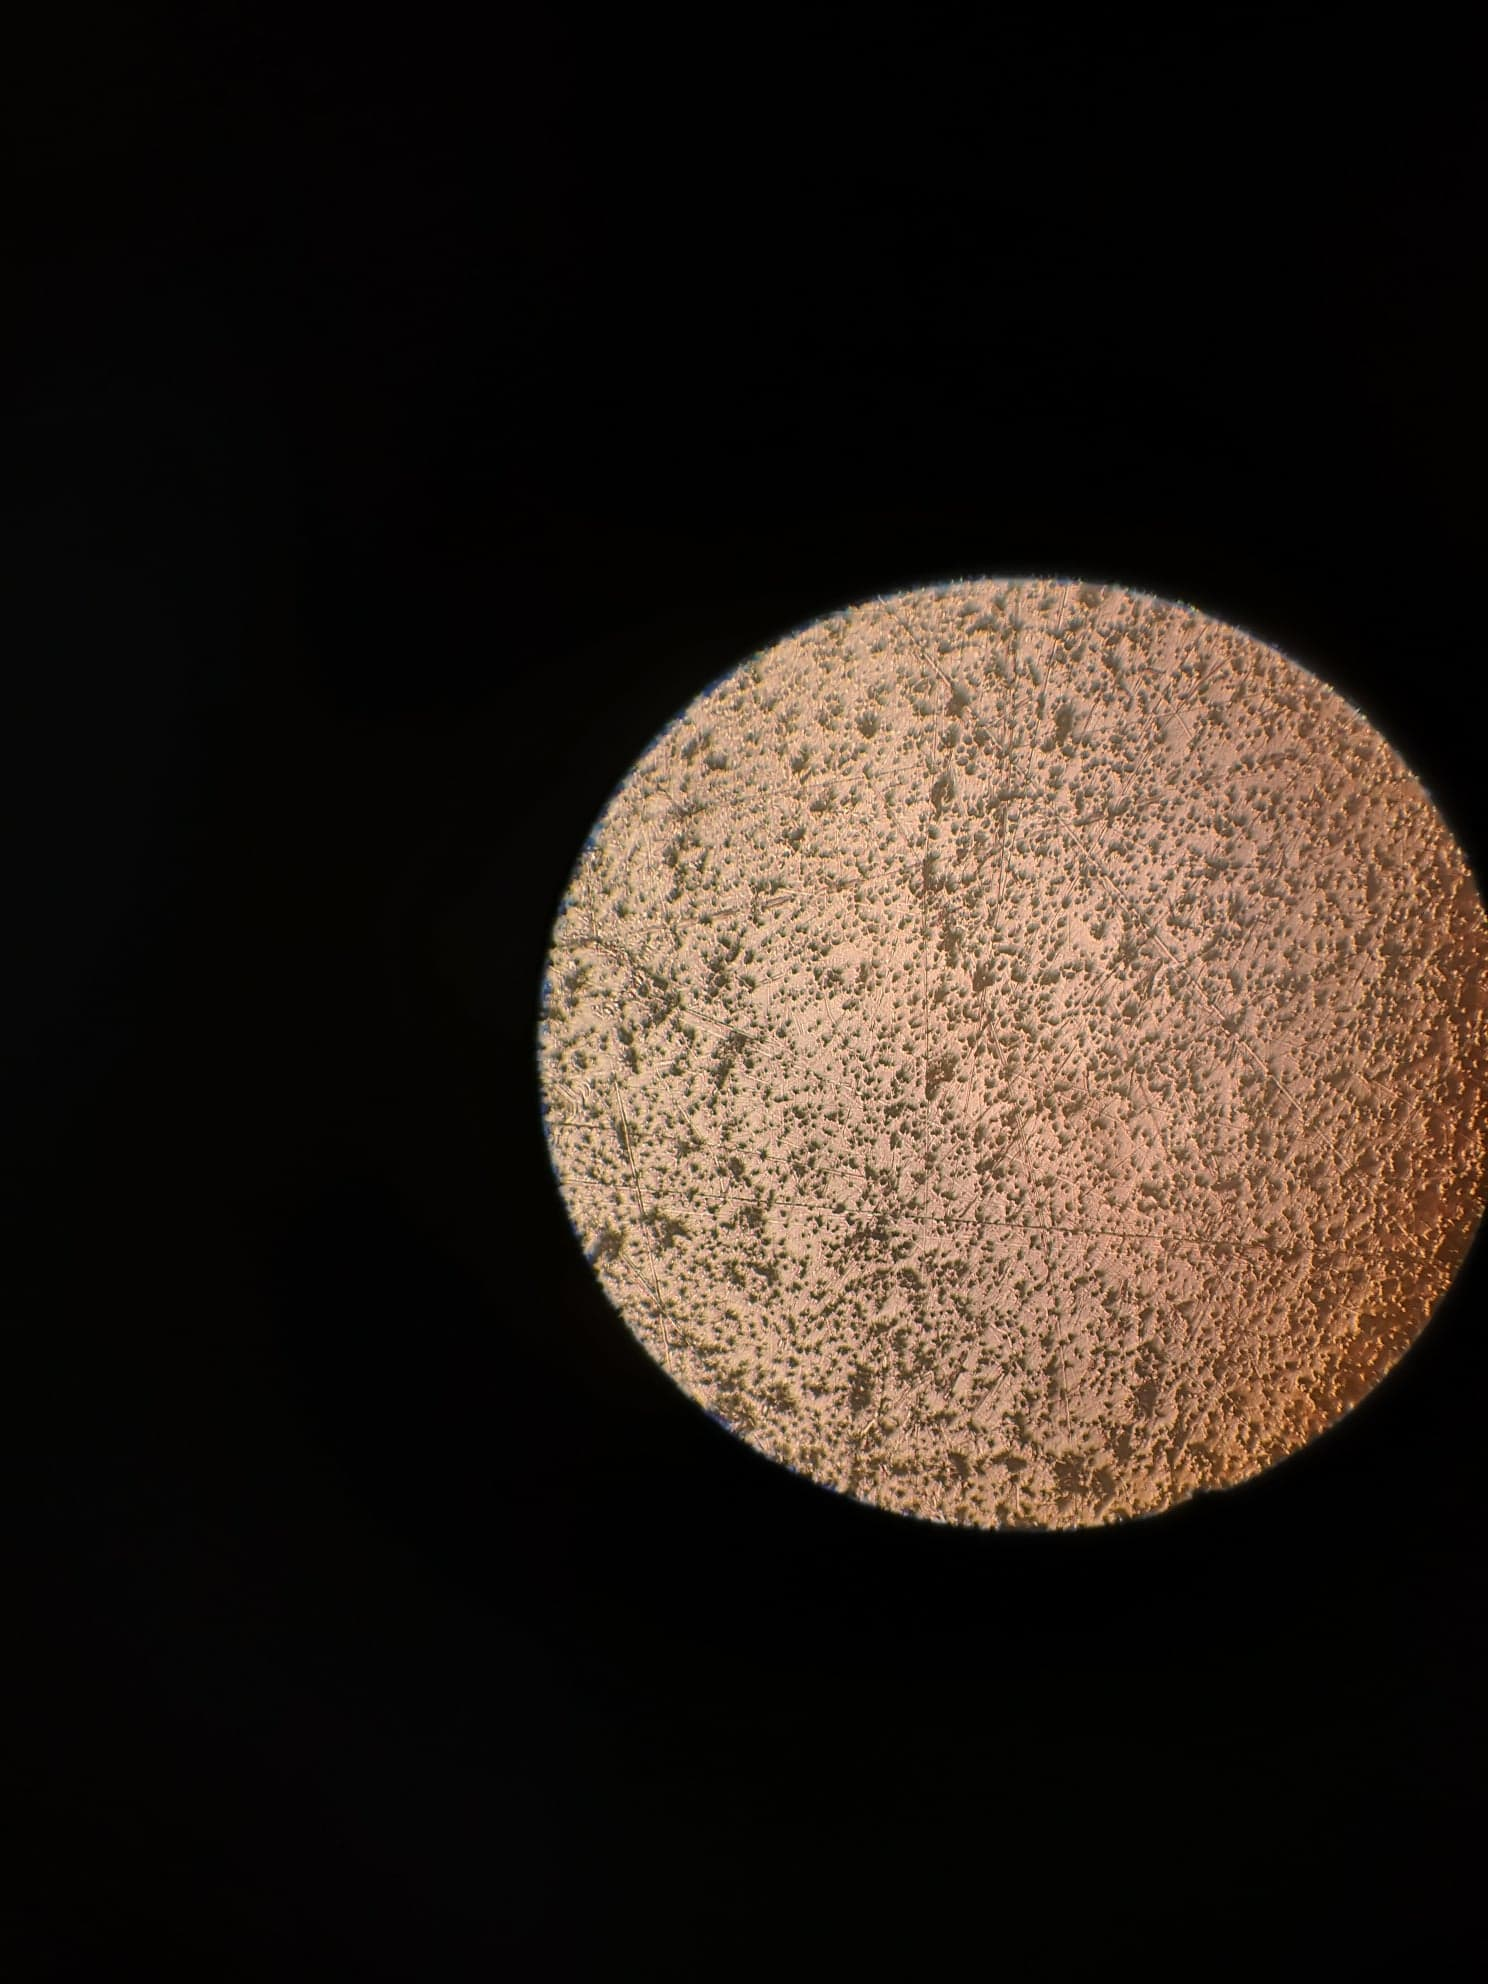
\includegraphics[width=.8\linewidth]{img/ferryt8.jpg}  
        \caption{Powiększenie $8x$}
    \end{subfigure}
    \begin{subfigure}{.5\textwidth}
        \centering
        % include second image
        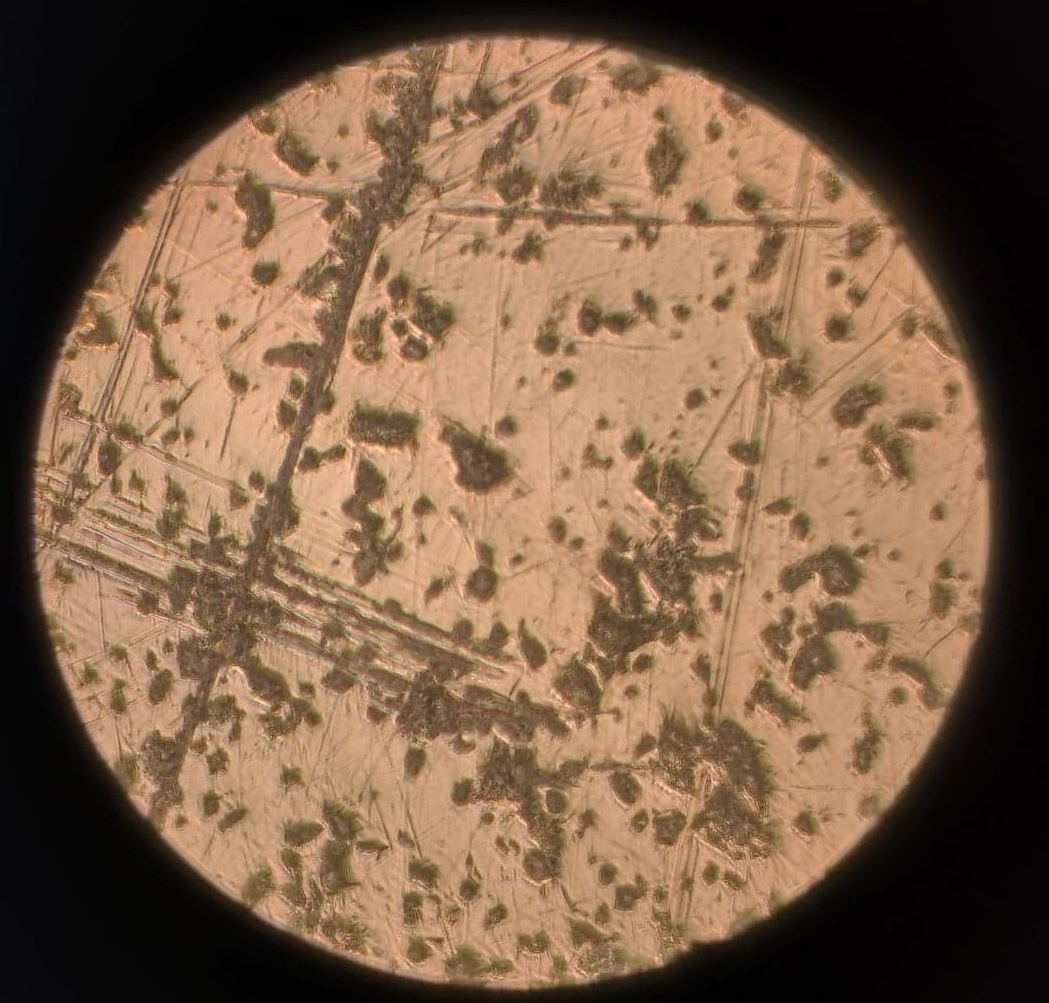
\includegraphics[width=.8\linewidth]{img/ferryt40.jpg}  
        \caption{Powiększenie $40x$}
    \end{subfigure}
    \caption{Ferryt}
\end{figure}

\begin{figure}[H]
    \begin{subfigure}{.5\textwidth}
        \centering
        % include first image
        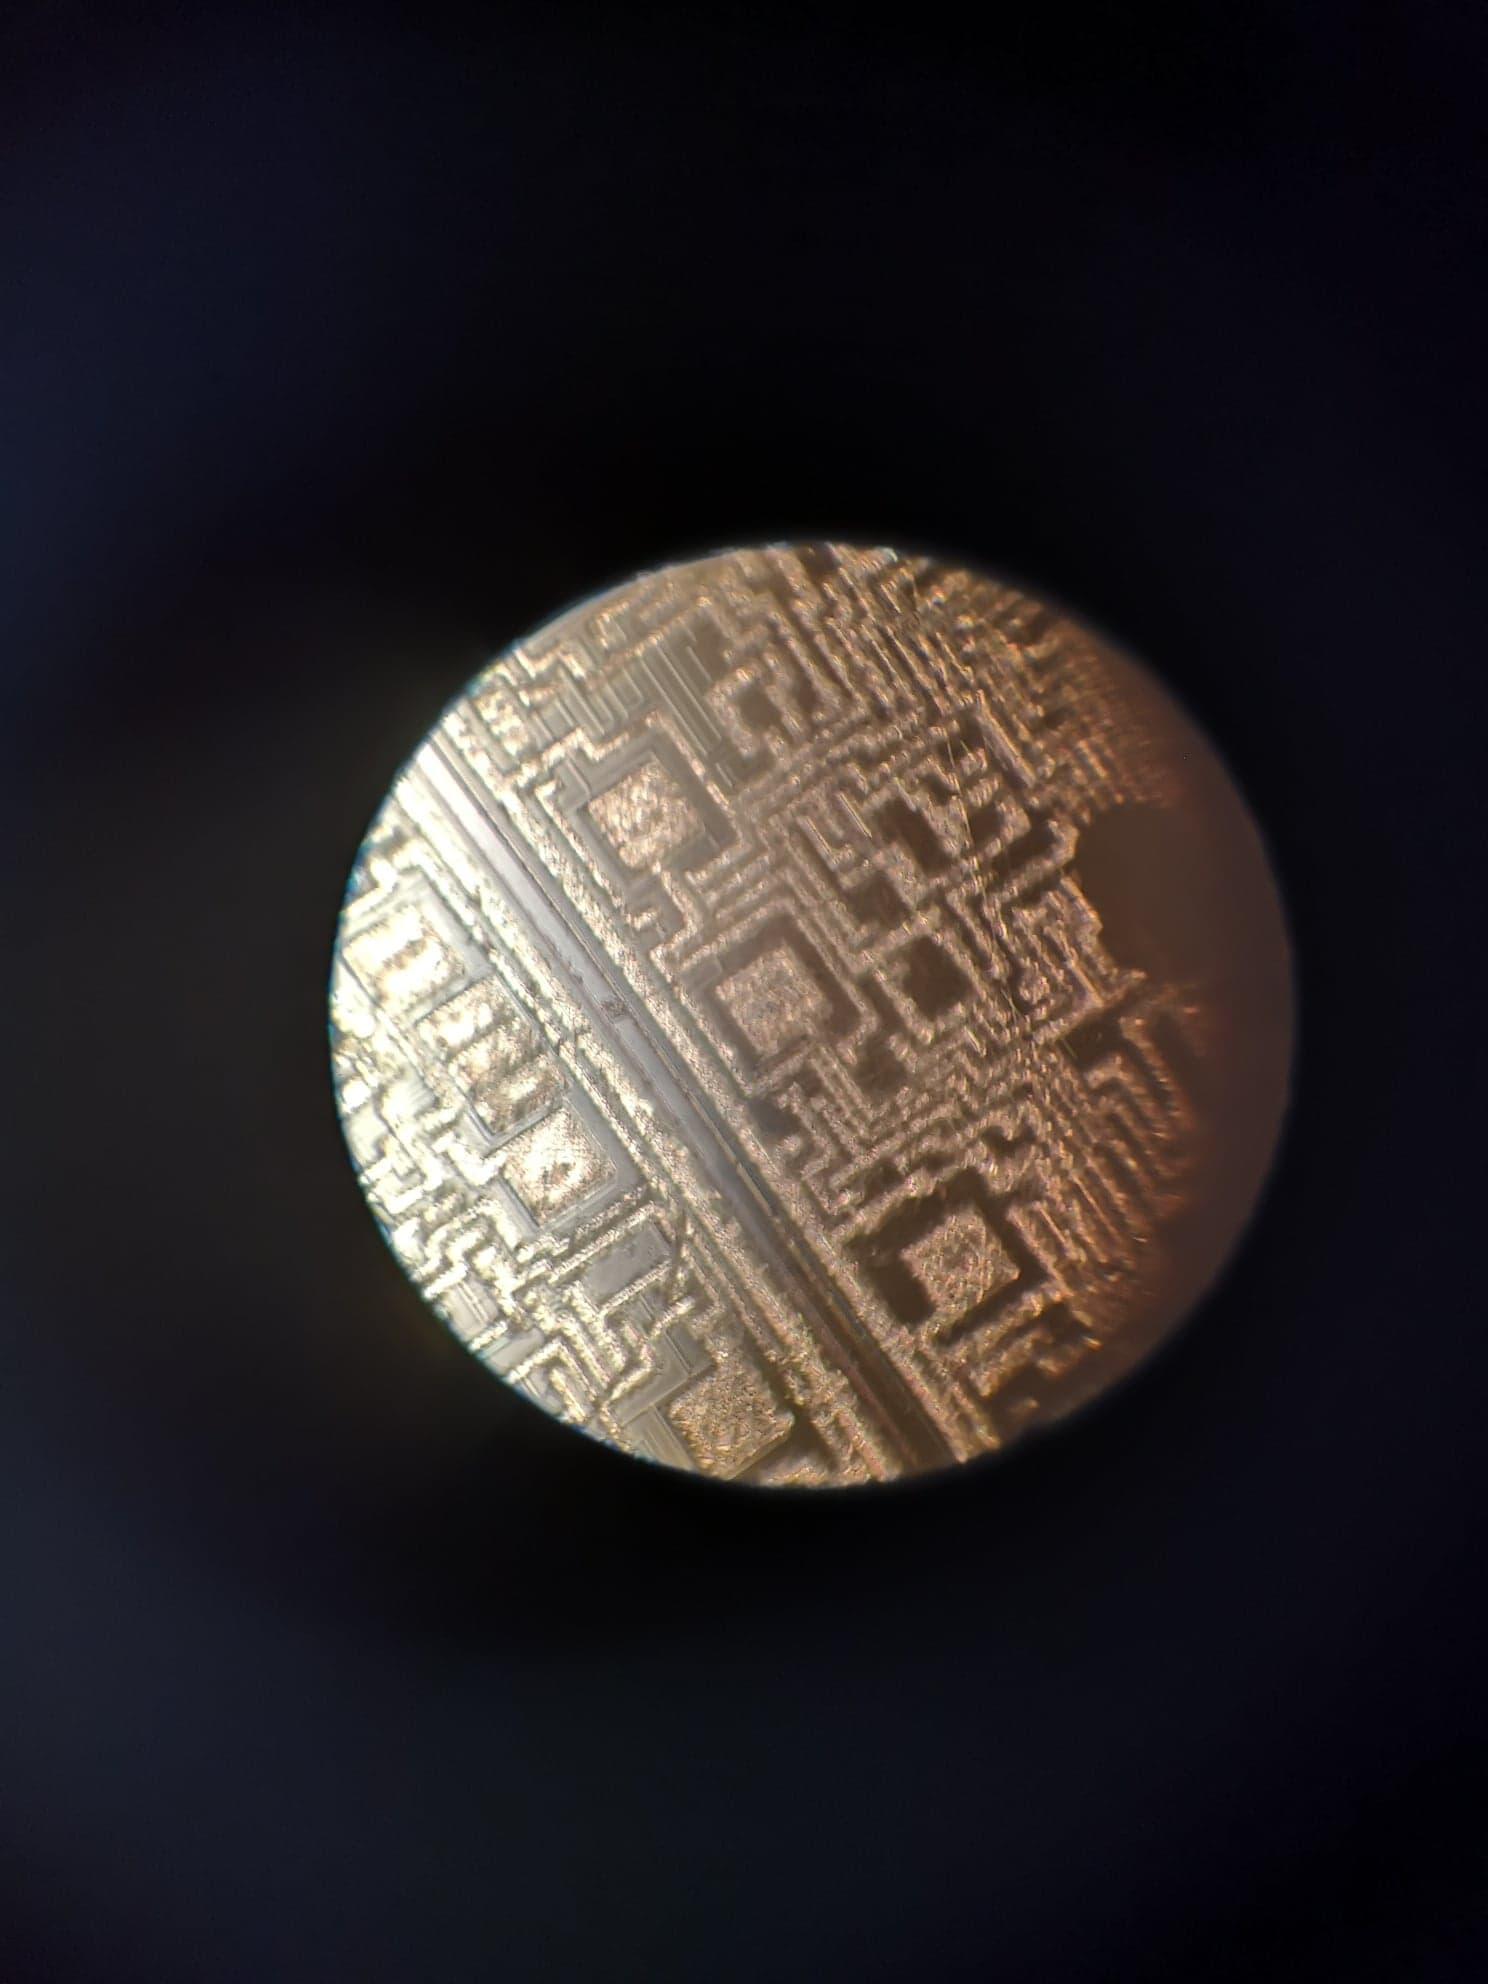
\includegraphics[width=.8\linewidth]{img/krzemowa8.jpg}  
        \caption{Powiększenie $8x$}
    \end{subfigure}
    \begin{subfigure}{.5\textwidth}
        \centering
        % include second image
        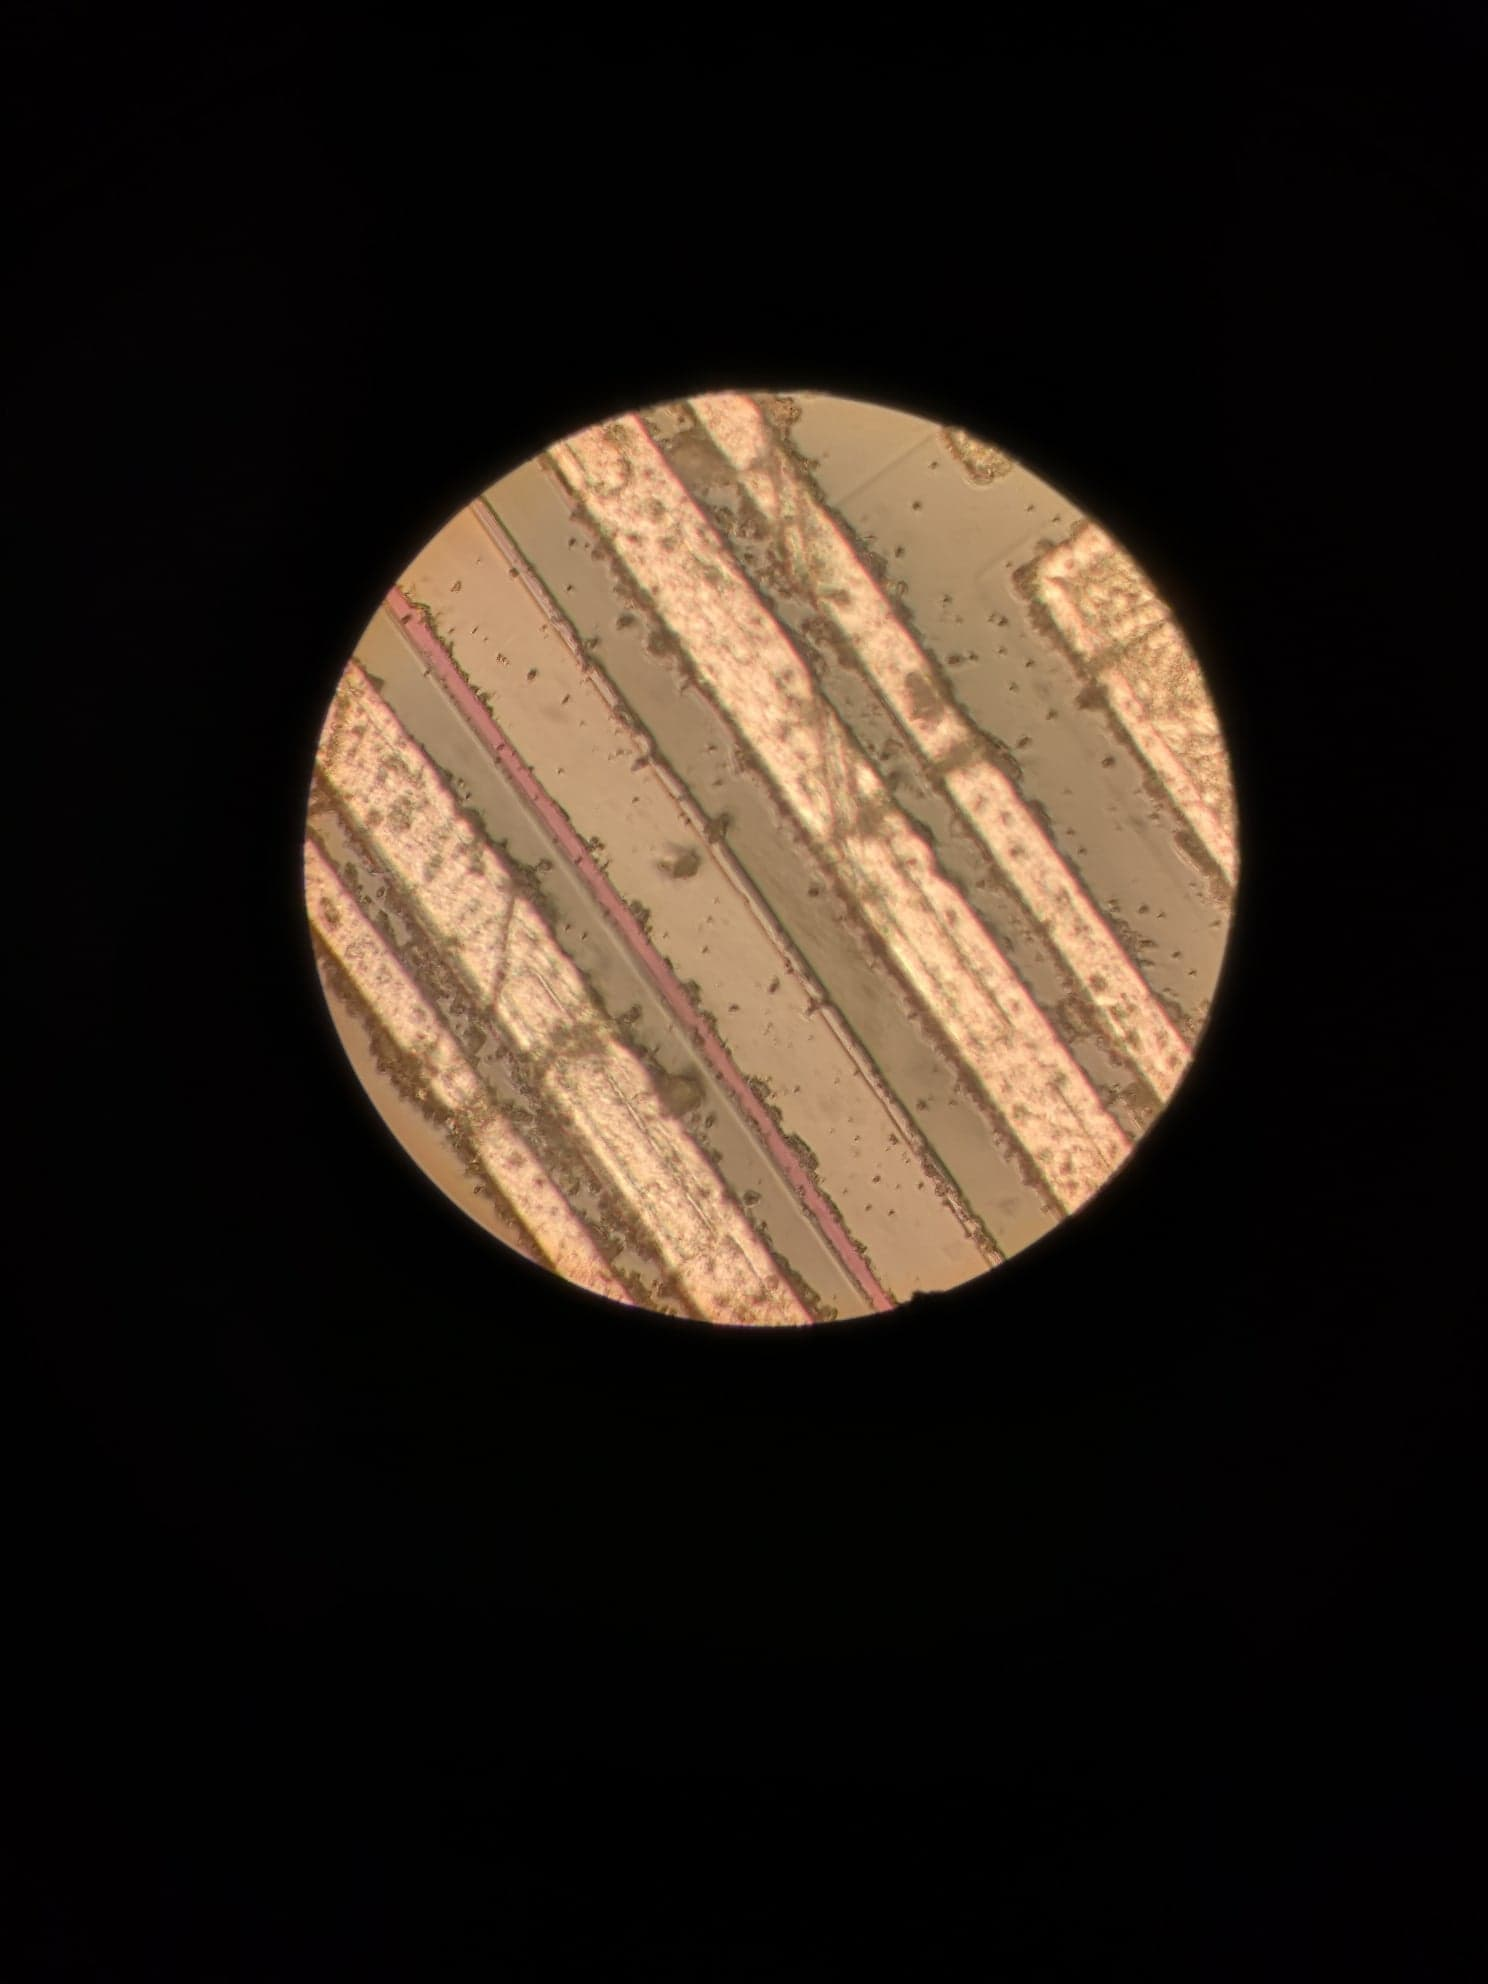
\includegraphics[width=.8\linewidth]{img/krzemowa40.jpg}  
        \caption{Powiększenie $40x$}
    \end{subfigure}
    \caption{Płytka krzemowa}
\end{figure}

\begin{figure}[H]
    \begin{subfigure}{.5\textwidth}
        \centering
        % include first image
        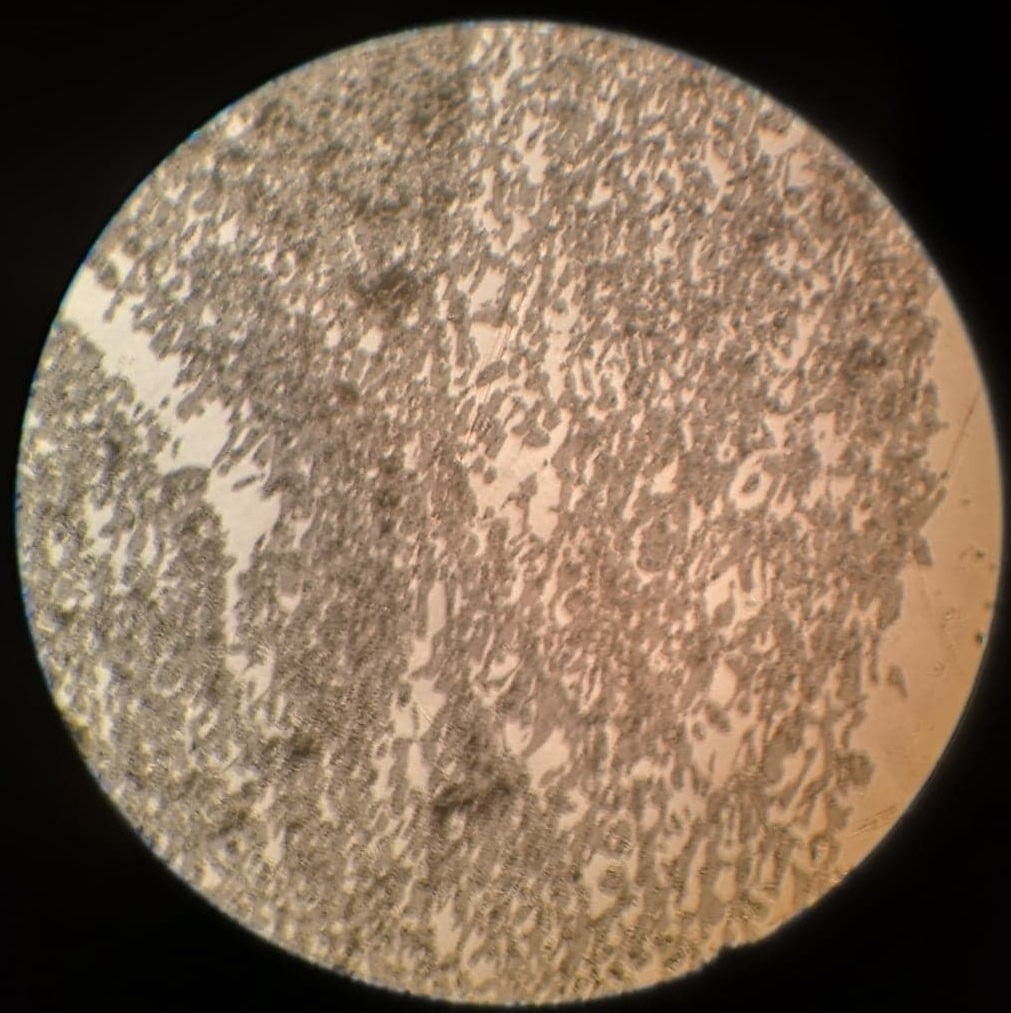
\includegraphics[width=.8\linewidth]{img/SiC-Si8.jpg}  
        \caption{Powiększenie $8x$}
    \end{subfigure}
    \begin{subfigure}{.5\textwidth}
        \centering
        % include second image
        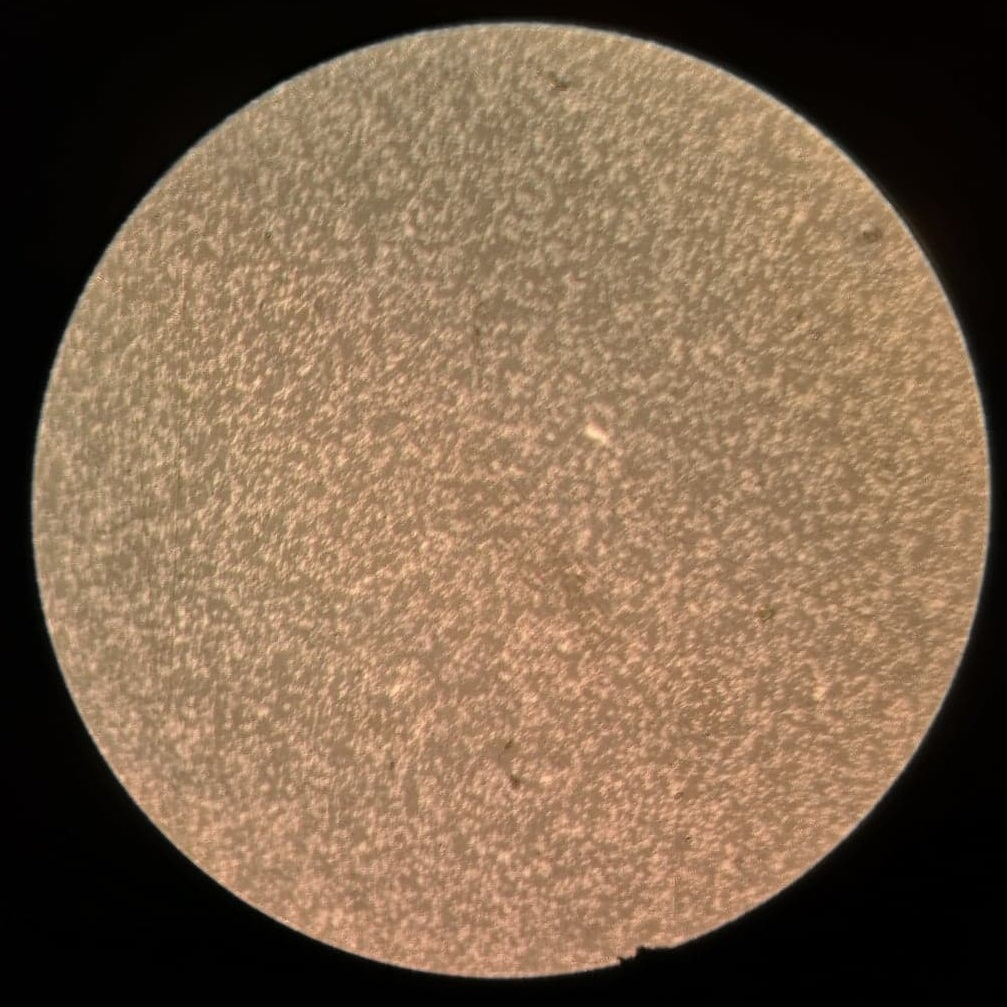
\includegraphics[width=.8\linewidth]{img/SiC-Si40.jpg}  
        \caption{Powiększenie $40x$}
    \end{subfigure}
    \caption{$SiC-Si$}
\end{figure}

\begin{figure}[H]
    \centering
    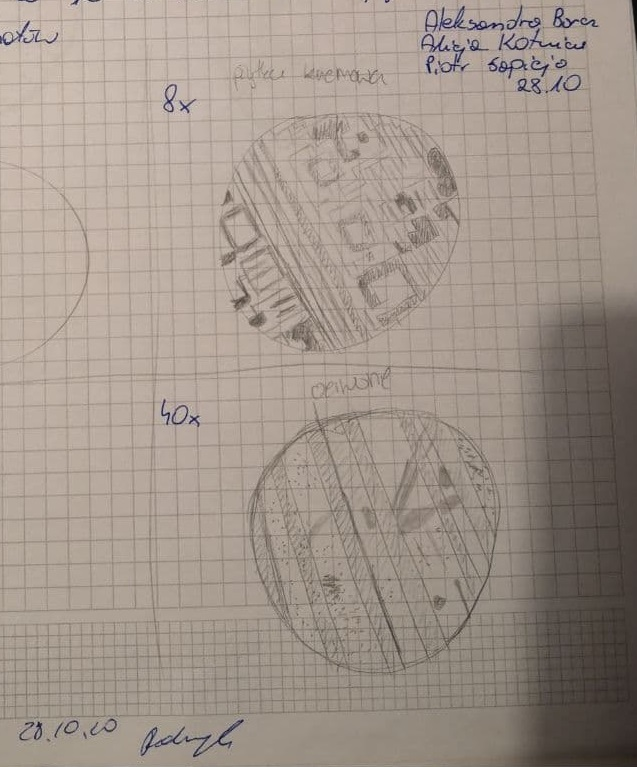
\includegraphics[width=0.6\textwidth]{img/schemat1.jpg}
    \caption{Schematy $1$.}
\end{figure}

\begin{figure}[H]
    \centering
    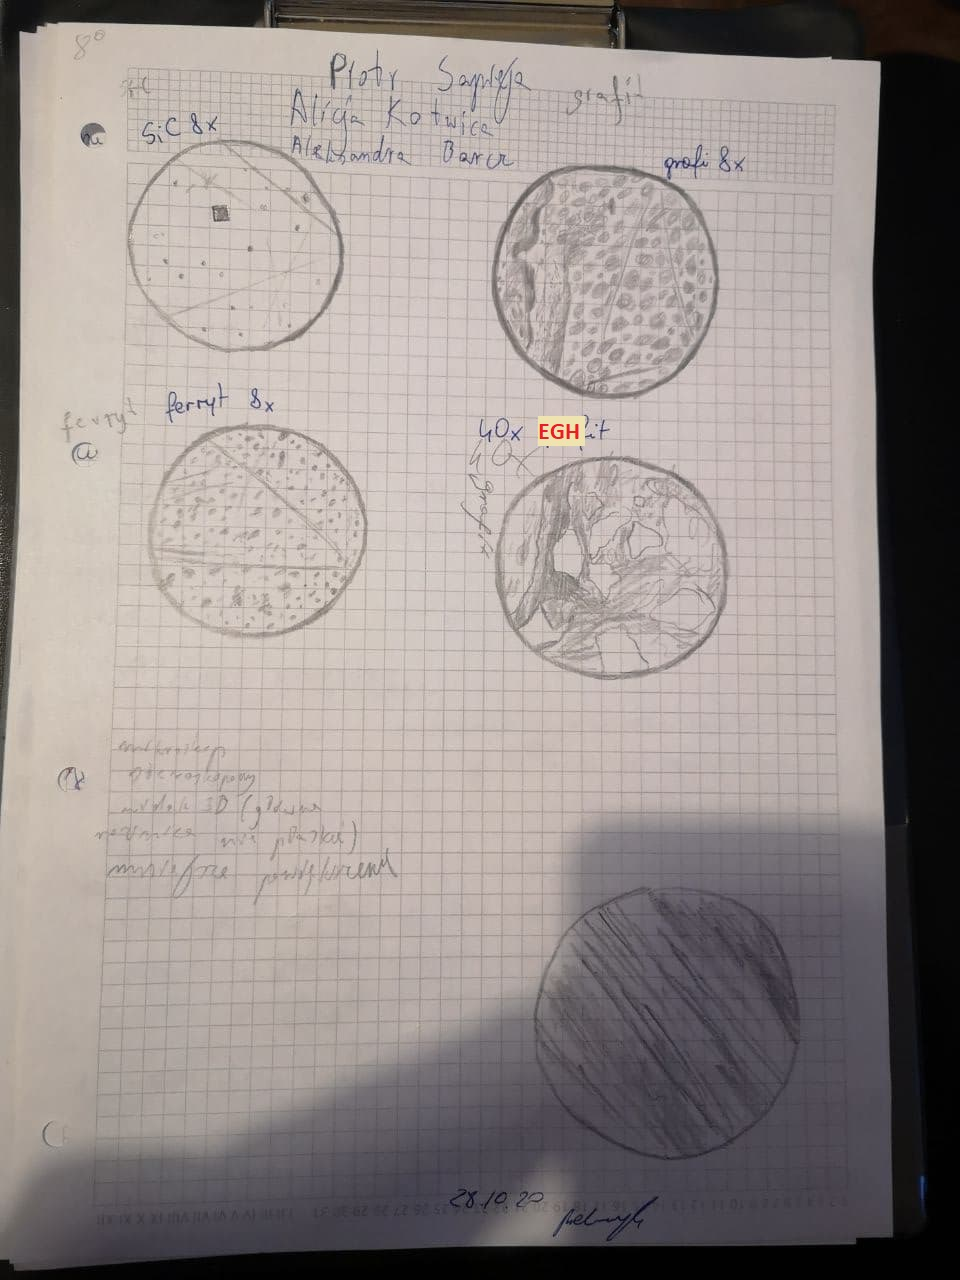
\includegraphics[width=0.7\textwidth]{img/schemat2.jpg}
    \caption{Schematy $2$.}
\end{figure}

\begin{figure}[H]
    \begin{subfigure}{.5\textwidth}
        \centering
        % include first image
        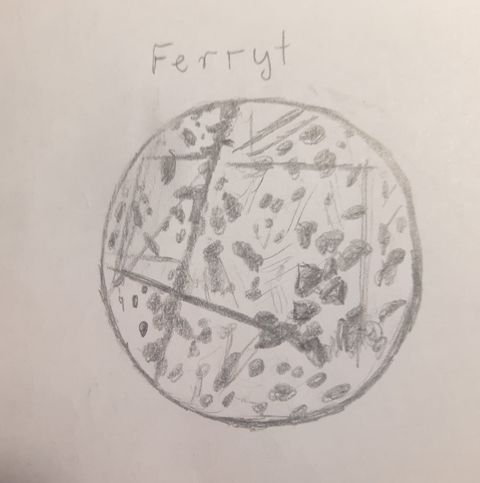
\includegraphics[width=.8\linewidth]{img/schemat_fer40.jpg}  
        \caption{Ferryt}
    \end{subfigure}
    \begin{subfigure}{.5\textwidth}
        \centering
        % include second image
        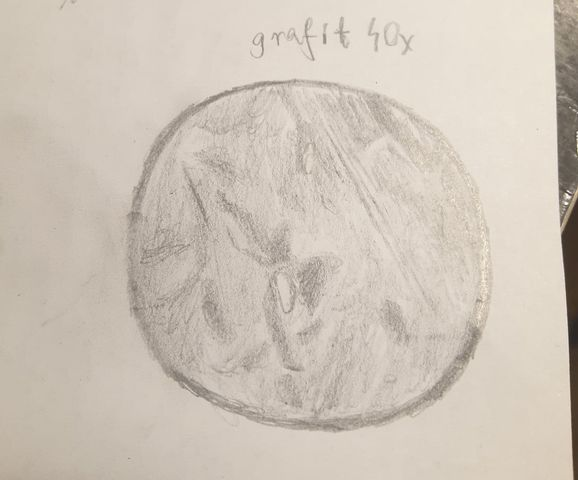
\includegraphics[width=.9\linewidth]{img/schemat_graf40.jpg}  
        \caption{Grafit}
    \end{subfigure}
    \caption{Schematy 3 w~powiększeniu $40x$ (naszkicowane już w~domu).}
\end{figure}

\begin{figure}[H]
    \begin{subfigure}{.5\textwidth}
        \centering
        % include first image
        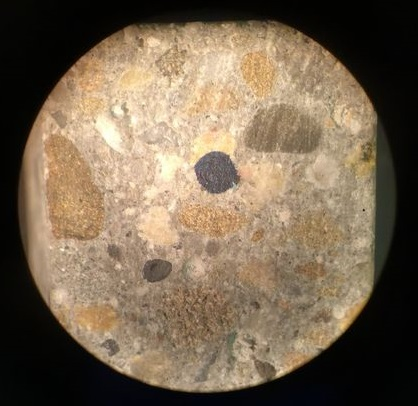
\includegraphics[width=.8\linewidth]{img/beton.jpg}  
        \caption{Beton}
    \end{subfigure}
    \begin{subfigure}{.5\textwidth}
        \centering
        % include second image
        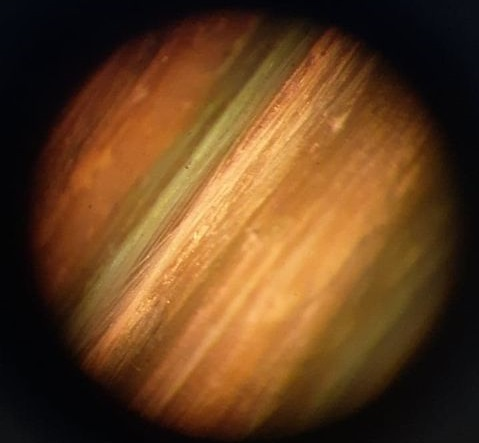
\includegraphics[width=.9\linewidth]{img/włókno.jpg}  
        \caption{Włókna szklane w~żywicy epoksydowej}
    \end{subfigure}
    \caption{Obraz próbek spod mikroskopu stereoskopowego.}
\end{figure}

\begin{figure}[H]
    \begin{subfigure}{.5\textwidth}
        \centering
        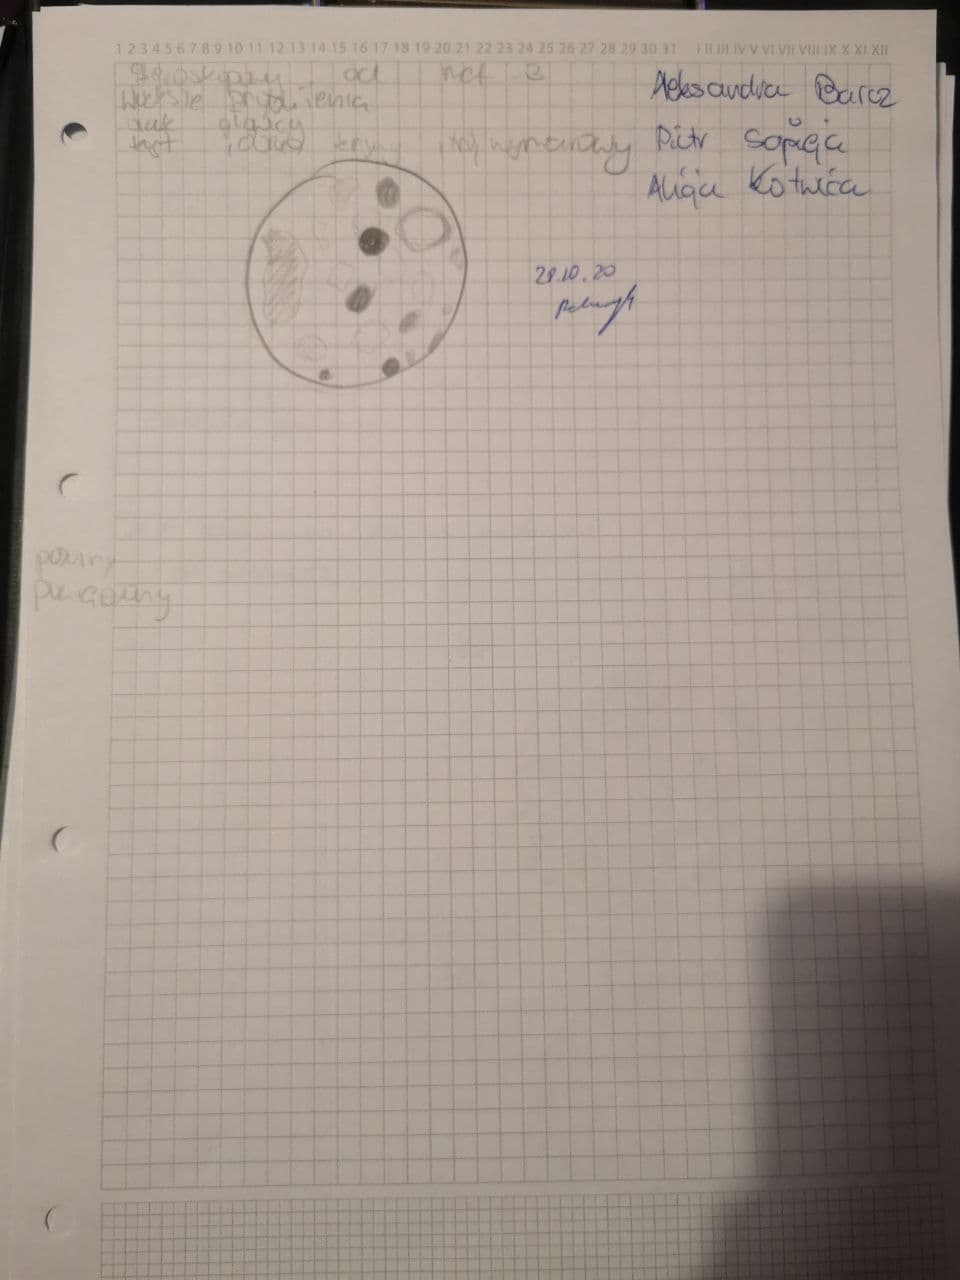
\includegraphics[width=.8\linewidth]{img/schemat3_bet.jpg}
        \caption{Schemat $1$}
    \end{subfigure}
    \begin{subfigure}{.5\textwidth}
        \centering
        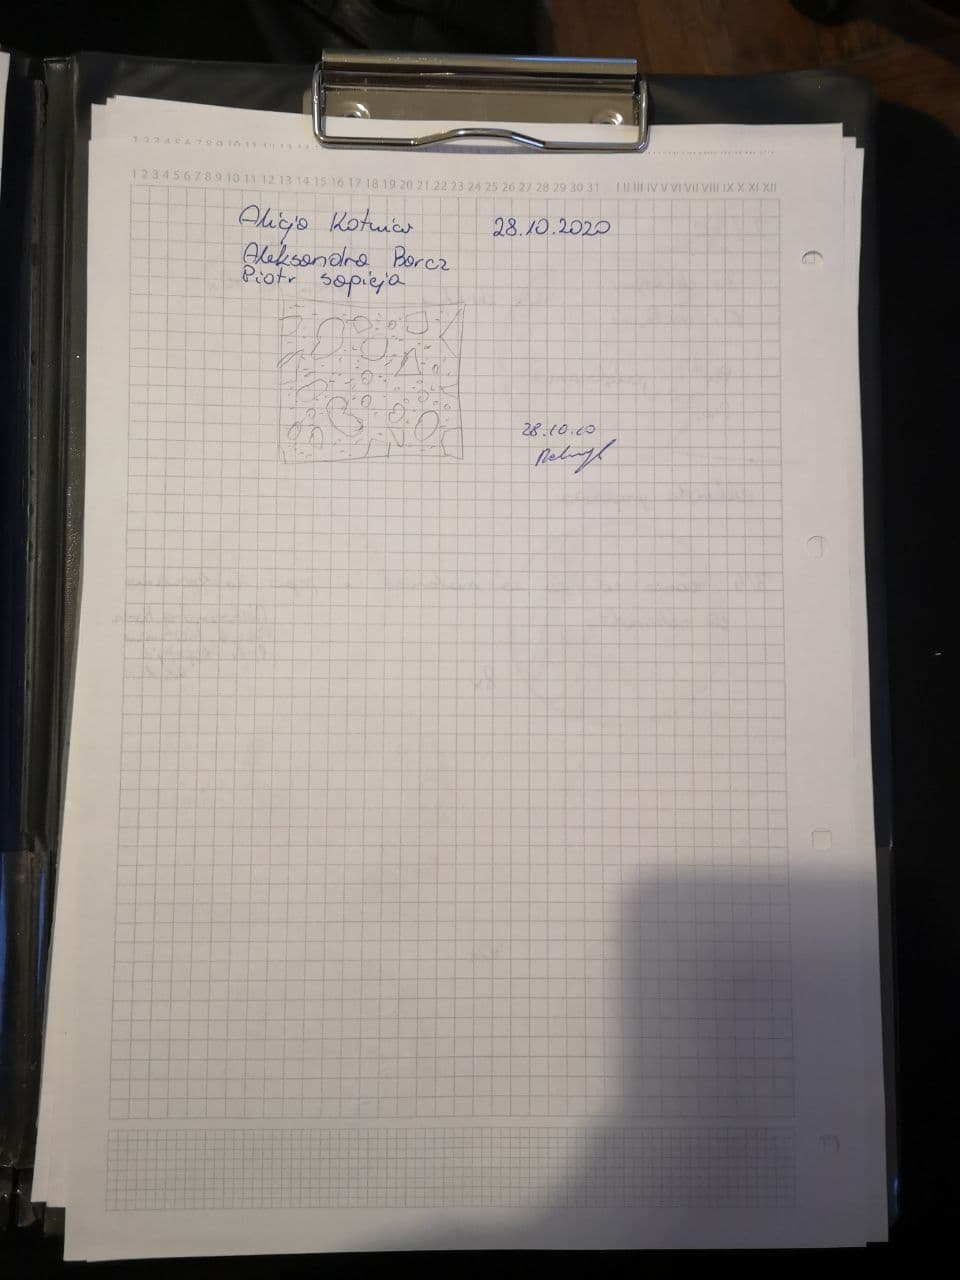
\includegraphics[width=.9\linewidth]{img/schemat4_bet.jpg}
        \caption{Schemat $2$}
    \end{subfigure}
    \caption{Schematy betonów z~mikroskopu stereoskopowego.}
\end{figure}

\begin{figure}[H]
    \centering
    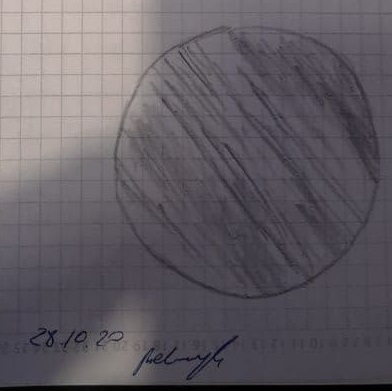
\includegraphics[width=0.7\textwidth]{img/schemat_ster_P.jpg}
    \caption{Schemat włókien szklanych w~żywicy epoksydowej z~mikroskopu stereoskopowego.}
\end{figure}

\end{document}
